\section{Communication options}

\frame{\tableofcontents[currentsection]}

\begin{frame}
    \frametitle{Options}
    \begin{itemize}
        \item \texttt{Node.spawn\_link}
        \item \texttt{:rpc} (Remote procedure calls)
        \item GenServer API
        \item Tasks
    \end{itemize}
\end{frame}

\begin{frame}
    \frametitle{\texttt{Node.spawn}}
    Spawns process outside of supervision trees (on other node). 
    
    \vfill

    This should be avoided at all costs.
\end{frame}

\begin{frame}
    \frametitle{\texttt{:rpc} (Remote procedure calls)}
    Example usage: \\
    \texttt{:rpc.call(:"foo@computer-name", Hello, :world, [])}
    \vfill
\end{frame}

\begin{frame}
    \frametitle{\texttt{:rpc} (Remote procedure calls)}
    Caveats: 
    \begin{itemize}
        \item Need to manually enter other node its name.
        \item Caller needs to know what modules are compiled on the other node.
        \item Executes a module function on a remote node. No global processes.
        \item Implies master-slave setup. (All knowing master executes code on slaves)
    \end{itemize}
\end{frame}

\begin{frame}
    \frametitle{GenServer API}
    Example usage: \\
    \texttt{GenServer.call(\{name, node\}, arg)}
    \vfill
\end{frame}

\begin{frame}
    \frametitle{GenServer API}
    Caveats: 
    \begin{itemize}
        \item Need to manually enter other node its name.
        \item Caller needs to know what genservers are running on the other node.
        \item Can't guarantee uniqueness of processes between nodes.
    \end{itemize}
\end{frame}


\begin{frame}
    \frametitle{Tasks (remote node spawning)}
    \begin{center}
        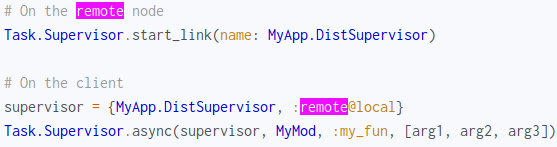
\includegraphics[scale=0.54]{03-remote-task.png}
    \end{center}
\end{frame}

\begin{frame}
    \frametitle{Tasks (remote node spawning)}
    Caveats: 
    \begin{itemize}
        \item Need to manually enter other node its name.
        \item Caller needs to know that there is a remote tasksupervisor
        \item Limited to tasks.
        \item Implies master-slave setup. (All knowing master starts tasks on slaves)
    \end{itemize}
\end{frame}

\begin{frame}
    \frametitle{So what do we want?}
    \begin{itemize}
        \item No need to enter node names manually
        \item No need to know what runs on which node
        \item We don't want to be limited to tasks
        \item No master-slave setup
    \end{itemize}
\end{frame}

